% Provenance (never printed): see sources/outline_sources.md (Year 2: radiogenic tracers
% Sr, Nd, Pb and mantle reservoirs; crustal growth; stable isotopes, delta notation and
% fractionation, d18O and d13C). Curves from figdata/bachelor-2/isotopes.py; exercise and
% problem values in the Book 4 scratch calculators calc/ch04.py and calc/ch04pb.py.
% Ruling (Sync 2): delta value and fractionation factor are chemistry's (Year 3 volume),
% recalled; this chapter defines the reference standards and the meteoric water line.
\chapter{الجيوكيمياء النظائرية}\label{ch:b2:isotope-geochemistry}

مانغايا، في جنوب المحيط الهادئ، وتريستان دا كونا، في جنوب المحيط
الأطلسي، جزيرتان بركانيتان مبنيتان من البازلت، وعيّنة يدوية من
إحداهما تشبه كثيرًا عيّنة يدوية من الأخرى، أو من ظهرة وسط محيطية.
لكن نظائرهما تميّز بينهما. فسترونشيوم بازلتات مانغايا يحمل
نسبة السترونشيوم 87 نفسها التي في الظهرات، أي نحو
$^{87}\mathrm{Sr}/^{86}\mathrm{Sr} = 0.7028$، بينما رصاصها من أكثر الرصاص
إشعاعيَّ المنشأ على الأرض، إذ تقارب فيه $^{206}\mathrm{Pb}/^{204}\mathrm{Pb}$ القيمة 21.6 مقابل
18.4 في الظهرات. أمّا بازلتات تريستان فتحوي سترونشيوم 87 أكثر، من 0.7050 إلى
0.7054، ونيوديميوم 143 أقل من كلتيهما. والانصهار لا يفرز نظائر
هذه العناصر الثقيلة، فتحمل كل حمم البصمة النظائرية
للوشاح الذي انصهر ليصنعها: فوشاح الأرض ليس خزّانًا واحدًا بل
عدة خزّانات، احتفظت بنسب مختلفة بين الأم والوليد مليارات
السنين. يستعمل هذا الفصل التحلّل الإشعاعي للروبيديوم والساماريوم واليورانيوم
والثوريوم مجموعةً من المقتفيات، ويتابع تطوّر الوشاح والقشرة
القارية عبر نظائر النيوديميوم، ويقسم الوشاح إلى
خزّانات ومزائج من الخزّانات، ويناقش سرعة نموّ القارات،
وينتهي بالنظائر المستقرة الخفيفة للأكسجين والهيدروجين والكربون، التي
تقتفي الماء والكربون عبر الأرض.
% ledger: data:b4-oib-isotopes, gale13:isotopes

\begin{recall}
تتحلّل الأم المشعّة بالمعدل $\lambda P$، وفي نظام مغلق تنمو نسبة
الوليد وفق $(D/D_s)_{\text{الآن}} = (D/D_s)_0 + (P/D_s)_{\text{الآن}}
(e^{\lambda t}-1)$، حيث $D_s$ نظير مستقر للوليد؛ والمعادن أو
الصخور التي تكوّنت معًا تقع على خط تساوٍ زمني، يعطي ميلُه العمر ويعطي
مقطعُه النسبةَ الابتدائية (مجلد المرحلة الثانوية، السنة الأخيرة؛ مجلد السنة الأولى،
فصل التأريخ الإشعاعي). ويفصل مطياف الكتلة الأيونات حسب نسبة
كتلتها إلى شحنتها (مجلد السنة الثانية من كتب الكيمياء). وقيمة $\delta$ لعيّنة
هي $\delta = (R_{\text{العيّنة}}/R_{\text{المعيار}} - 1)\times 1000$، بالجزء في
الألف، ومعامل التجزّؤ بين طورين A وB هو
$\alpha_{\mathrm{A/B}} = R_{\mathrm A}/R_{\mathrm B}$، حيث $R$ نسبة النظير
الثقيل إلى الخفيف؛ وقد قُدّم كلاهما، مع طاقات نقطة الصفر
التي تسبّب التجزّؤ النظائري، في مجلد السنة الثالثة من كتب الكيمياء.
وقد عُرّفت العناصر غير المتوافقة وبازلت MORB وبازلت OIB في
\cref{ch:b2:elements-in-the-earth}.
\end{recall}

\section{النظائر المشعّة المنشأ مقتفياتٍ}

تحمل ثلاثة أنظمة تحلّل معظم المعلومات عن الوشاح والقشرة.
فالروبيديوم 87 يتحلّل إلى السترونشيوم 87، والساماريوم 147 إلى النيوديميوم 143، واليورانيوم
والثوريوم، عبر سلاسل تحلّلهما، إلى ثلاثة نظائر للرصاص. وتختلف كل أم
ووليدها في سلوكهما أثناء الانصهار، ولكل وليد نظير
مستقر غير مشعّ المنشأ يُقاس بالنسبة إليه.

\begin{table}[ht]
\centering
\begin{tabular}{lllll}
\hline
الأم & الوليد & النسبة المقيسة & ثابت التحلّل (لكل سنة) & عمر النصف (Ga)\\
\hline
$^{87}$Rb & $^{87}$Sr & $^{87}\mathrm{Sr}/^{86}\mathrm{Sr}$ & \num{1.3972e-11} & 49.6\\
$^{147}$Sm & $^{143}$Nd & $^{143}\mathrm{Nd}/^{144}\mathrm{Nd}$ & \num{6.524e-12} & 106.25\\
$^{238}$U & $^{206}$Pb & $^{206}\mathrm{Pb}/^{204}\mathrm{Pb}$ & \num{1.55125e-10} & 4.47\\
\hline
\end{tabular}
\caption{ثلاثة أنظمة تحلّل طويلة العمر تُستعمل مقتفياتٍ. البيانات: توصيات
\babelsublr{IUPAC--IUGS} (فيلا وآخرون، 2020 و2022).}
\label{tab:b2:isotope-geochemistry:decay}
\end{table}
% ledger: villa22:rb87, villa20:sm147

\begin{definition}[المقتفي النظائري المشعّ المنشأ]\label{def:b2:isotope-geochemistry:tracer}
\emph{المقتفي النظائري المشعّ المنشأ}\index{المقتفي النظائري المشعّ المنشأ} هو نسبة
نظير وليد تنتجه أم مشعّة طويلة العمر إلى نظير مستقر
من العنصر نفسه، مثل $^{87}\mathrm{Sr}/^{86}\mathrm{Sr}$ أو
$^{143}\mathrm{Nd}/^{144}\mathrm{Nd}$، تُستعمل لتعرّف مصدر الصخر لا
لتأريخه. وتنمو نسبة الخزّان بمعدل يحدّده نسبة
الأم إلى الوليد فيه، فتسجّل تاريخ تلك النسبة.
\end{definition}

ينفصل عنصرا زوج التحلّل كلما انصهر الوشاح. ففي
\cref{ch:b2:elements-in-the-earth} تبيّن أن الروبيديوم أشدّ عدمَ توافق من
السترونشيوم، وأن النيوديميوم أشدّ عدمَ توافق من الساماريوم. فالمصهور، والقشرة
التي يبنيها، يغادران الوشاح إذن بنسبة Rb/Sr عالية ونسبة Sm/Nd منخفضة؛ ويحتفظ
المتبقّي بنسبة Rb/Sr منخفضة ونسبة Sm/Nd عالية. ومع الزمن تكتسب القشرة
السترونشيوم 87 أسرع من مصدرها والنيوديميوم 143 أبطأ منه؛ ويفعل \omterm{def:b2:isotope-geochemistry:reservoirs}{الوشاح
المستنزَف} العكس. فتتحرّك نسب الزوجين في اتجاهين
متعاكسين، وهي نقطة يوضّحها مخطّط Sr--Nd أدناه.

\begin{proposition}[النسب النظائرية تصمد أمام الانصهار]\label{prop:b2:isotope-geochemistry:melting}
حين ينصهر صخر وينفصل المصهور عن المتبقّي، تساوي نسبتا
$^{87}\mathrm{Sr}/^{86}\mathrm{Sr}$ و$^{143}\mathrm{Nd}/^{144}\mathrm{Nd}$ في
المصهور نظيرتيهما في المصدر في حدود دقة
القياسات؛ ولا تتغيّر إلا نسب الأم إلى الوليد، Rb/Sr وSm/Nd.
\end{proposition}
\admitted

\noindent تقوم هذه المقولة على حقيقتين. فلنظائر العنصر الواحد البنية
الإلكترونية نفسها، فتدخل البلّورة أو المصهور بالتساوي تقريبًا؛ والفرق
النسبي في الكتلة بين السترونشيوم 87 والسترونشيوم 86، نحو واحد في
المئة، أصغر بكثير منه للأكسجين أو الهيدروجين، وعند درجة الحرارة العالية يتناقص
لوغاريتم معامل التجزّؤ التوازني تناسبًا مع مقلوب مربع
درجة الحرارة، فيقترب المعامل من 1. ثم إن القياس نفسه يصحّح
التجزّؤ الذي يحدث في مطياف الكتلة بتثبيت نسبة نظيرين
غير مشعّي المنشأ (للنيوديميوم، $^{146}\mathrm{Nd}/^{144}\mathrm{Nd} =
0.7219$)، وهذا يمحو أيضًا أي تجزّؤ طبيعي صغير. فالحمم إذن
تأخذ عيّنة من النسب النظائرية لمصدرها، بينما تعكس نسب عناصرها
النزرة الانصهار أيضًا.
% ledger: white:chur, white:t-dependence

\section{تطوّر الوشاح والقشرة}

\subsection{الخزّان الكوندريتي}

الساماريوم والنيوديميوم كلاهما من \omterm{def:b2:elements-in-the-earth:ree}{العناصر الأرضية النادرة} المحبّة للصخور العصيّة على التبخّر
(\cref{ch:b2:elements-in-the-earth}): فينبغي أن تكون \omterm{def:b2:elements-in-the-earth:bse}{الأرض السيليكاتية الكلية} قد احتفظت
بنسبتهما الكوندريتية. وتعطي الكوندريتات إذن تاريخ Sm--Nd للأرض
غير المتمايزة.

\begin{definition}[الخزّان الكوندريتي المنتظم]\label{def:b2:isotope-geochemistry:chur}
\emph{الخزّان الكوندريتي المنتظم}\index{الخزّان الكوندريتي المنتظم}
(CHUR) خزّان نموذجي له تركيب الساماريوم والنيوديميوم في
الكوندريتات، مغلق منذ تكوّن المجموعة الشمسية. ونسبتاه
الحاليتان $(^{143}\mathrm{Nd}/^{144}\mathrm{Nd})_{\mathrm{CHUR}} = 0.512638$
و$(^{147}\mathrm{Sm}/^{144}\mathrm{Nd})_{\mathrm{CHUR}} = 0.1966$.
\end{definition}
% ledger: white:chur

بتشغيل معادلة التساوي الزمني إلى الوراء، كانت للخزّان CHUR، حين تكاثفت أولى المواد الصلبة
قبل \qty{4567}{Myr} (\cref{ch:b2:planet-formation-meteorites})، النسبة
\[
  ^{143}\mathrm{Nd}/^{144}\mathrm{Nd} = 0.512638 - 0.1966\,\bigl(e^{\lambda\cdot
  \num{4.567e9}\,\mathrm{yr}}-1\bigr) = 0.506692 .
\] ومنذ ذلك الحين ازدادت نسبته بمقدار
1.2 في المئة. والفروق بين صخور الأرض أصغر بألف مرة،
وتُذكر بوحدة أنسب.
% ledger: lugaro:cai, villa20:sm147

\begin{definition}[ترميز إبسيلون]\label{def:b2:isotope-geochemistry:epsilon}
\emph{ترميز إبسيلون}\index{ترميز إبسيلون} يعبّر عن نسبة
$^{143}\mathrm{Nd}/^{144}\mathrm{Nd}$ لعيّنة، في زمن $t$ قبل
الحاضر، بانحرافها النسبي عن CHUR في الزمن نفسه، بالجزء من عشرة
آلاف:
\[
  \varepsilon_{\mathrm{Nd}}(t) = \left(
  \frac{(^{143}\mathrm{Nd}/^{144}\mathrm{Nd})_{\text{العيّنة}}(t)}
       {(^{143}\mathrm{Nd}/^{144}\mathrm{Nd})_{\mathrm{CHUR}}(t)} - 1\right)\times 10^4 .
\]
ومن دون ذكر الزمن، $\varepsilon_{\mathrm{Nd}}$ هي القيمة الحالية.
\end{definition}

لبازلت MORB المتوسط، الذي فيه $^{143}\mathrm{Nd}/^{144}\mathrm{Nd} = 0.513074$،
$\varepsilon_{\mathrm{Nd}} = (0.513074/0.512638 - 1)\times10^4 = +8.5$؛ ومعظم الصخور
يقع بين $-20$ و$+10$. والقيمة الموجبة تعني أن مصدر الصخر
كانت له، في المتوسط على مدى تاريخ الأرض، نسبة Sm/Nd أعلى من
الكوندريتات: فهو مستنزف في العنصر الأشدّ عدمَ توافق، أي النيوديميوم.
والقيمة السالبة تعني العكس. ويُقاس الابتعاد عن نسبة Sm/Nd الكوندريتية
بالانحراف الكسري
\[
  f_{\mathrm{Sm/Nd}} = \frac{(\mathrm{Sm}/\mathrm{Nd})_{\text{العيّنة}}}
  {(\mathrm{Sm}/\mathrm{Nd})_{\mathrm{CHUR}}} - 1,
\]
وهو هو سواء أكانت النسب كتلية أم ذرّية. ومع قيم CI
في \cref{ch:b2:elements-in-the-earth} (Sm 0.145، Nd \qty{0.457}{ppm}،
$\mathrm{Sm}/\mathrm{Nd} = 0.317$)، يكون للقشرة القارية العلوية (4.7
و\qty{27}{ppm}، 0.174) $f_{\mathrm{Sm/Nd}} = -0.45$.
% ledger: gale13:isotopes, white:chur, lodders:ci-table, rg03:ucc-trace

\begin{proposition}[النموّ الخطي للقيمة $\varepsilon_{\mathrm{Nd}}$]\label{prop:b2:isotope-geochemistry:linear}
الخزّان الذي انفصل عن CHUR واحتفظ منذ ذلك الحين بالانحراف الكسري
$f_{\mathrm{Sm/Nd}}$ تتغيّر قيمة $\varepsilon_{\mathrm{Nd}}$ فيه، مع تقدّم
الزمن، بالمعدل
\[
  \frac{\mathrm{d}\varepsilon_{\mathrm{Nd}}}{\mathrm{d}\tau} \approx Q\,f_{\mathrm{Sm/Nd}},
  \qquad
  Q = 10^4\,\lambda_{147}\,
  \frac{(^{147}\mathrm{Sm}/^{144}\mathrm{Nd})_{\mathrm{CHUR}}}
       {(^{143}\mathrm{Nd}/^{144}\mathrm{Nd})_{\mathrm{CHUR}}}
  = \qty{25.0}{\per\giga\year},
\]
حيث $\tau$ الزمن معدودًا إلى الأمام. فالخزّان الذي كانت له $\varepsilon_0$ عند
انفصاله، قبل زمن $T$، تكون له اليوم $\varepsilon_{\mathrm{Nd}} \approx \varepsilon_0
+ Q f_{\mathrm{Sm/Nd}} T$.
\end{proposition}

\begin{proof}
لنكتب $R$ بدل $^{143}\mathrm{Nd}/^{144}\mathrm{Nd}$ و$p$ بدل
$^{147}\mathrm{Sm}/^{144}\mathrm{Nd}$. في خزّان مغلق
$\mathrm{d}R/\mathrm{d}\tau = \lambda p\,e^{\lambda t}$، حيث $t$ الزمن قبل
الحاضر؛ وبما أن $\lambda t \le 0.03$، فإن العامل $e^{\lambda t}$ يختلف عن 1 بما لا يزيد على
3 في المئة، و$\mathrm{d}R/\mathrm{d}\tau \approx \lambda p$. ومنه
$\mathrm{d}(R_s - R_c)/\mathrm{d}\tau \approx \lambda (p_s - p_c) = \lambda p_c
f_{\mathrm{Sm/Nd}}$، لأن $p_s/p_c - 1 = f_{\mathrm{Sm/Nd}}$. والقسمة على $R_c$،
الذي لا يتغيّر إلا بنسبة 1.2 في المئة على مدى عمر الأرض، تعطي
$\mathrm{d}\varepsilon/\mathrm{d}\tau \approx 10^4\lambda p_c f/R_c$. ومع
$\lambda = \qty{6.524e-12}{\per\year}$ و$p_c = 0.1966$ و$R_c = 0.512638$، يكون $Q =
\num{2.502e-8}$ لكل سنة، أي \qty{25.0}{\per\giga\year}.
\end{proof}
% ledger: villa20:sm147, white:chur

فالقشرة التي لها نسبة Sm/Nd القشرة العلوية ($f = -0.45$) تفقد إذن نحو
11 وحدة إبسيلون في كل مليار سنة نسبةً إلى CHUR، بينما لا يحتاج خزّان
وشاحي إلا إلى $f = +0.07$ ليصعد من 0 إلى قيمة MORB البالغة $+8.5$ في
\qty{4.567}{Ga}. ويتتبّع الشكل أدناه المعادلات الدقيقة لثلاثة
خزّانات: CHUR، ووشاح مستنزَف مغلق منذ تكوّن الأرض بنسبة Sm/Nd
التي توصله إلى قيمة MORB اليوم ($^{147}\mathrm{Sm}/^{144}\mathrm{Nd} =
0.211$)، وقشرة استُخلصت من ذلك الوشاح قبل 2.7 مليار سنة بنسبة Sm/Nd
القشرة العلوية ($0.108$). وقد بدأت القشرة عند $\varepsilon_{\mathrm{Nd}} =
+3.5$، وهي قيمة مصدرها في ذلك الحين، وهي الآن عند $-27$.

\begin{definition}[الوشاح المستنزَف، الوشاح المُثرى]\label{def:b2:isotope-geochemistry:reservoirs}
\emph{الوشاح المستنزَف}\index{الوشاح المستنزَف} جزء من الوشاح
فقد عناصر غير متوافقة لصالح المصاهير، فصارت نسبة Sm/Nd فيه أعلى ونسبة Rb/Sr
أدنى من الكوندريتية؛ ومع الزمن تصير $\varepsilon_{\mathrm{Nd}}$ فيه موجبة
و$^{87}\mathrm{Sr}/^{86}\mathrm{Sr}$ منخفضة. و\emph{الوشاح
المُثرى}\index{الوشاح المُثرى} جزء من الوشاح اكتسب
عناصر غير متوافقة، من قشرة معاد تدويرها مثلًا أو من مصاهير صغيرة،
وله $\varepsilon_{\mathrm{Nd}}$ سالبة أو $^{87}\mathrm{Sr}/^{86}\mathrm{Sr}$ عالية.
\end{definition}

\begin{omfigure}
\centering
\begin{tikzpicture}
\begin{axis}[omrecord, width=0.82\linewidth, height=6.4cm,
  x dir=reverse, xmin=0, xmax=4.6, ymin=-30, ymax=12,
  xlabel={\foreignlanguage{arabic}{الزمن قبل الحاضر \babelsublr{(Ga)}}}, ylabel={$\varepsilon_{\mathrm{Nd}}(t)$},
  tick label style={font=\scriptsize}, label style={font=\small}]
\addplot[thick, black] table[x=t_Ga, y=eps] {figdata/out/bachelor-2-isotopes-chur.dat};
\addplot[very thick, blue!70!black] table[x=t_Ga, y=eps] {figdata/out/bachelor-2-isotopes-dm.dat};
\addplot[very thick, brown!70!black] table[x=t_Ga, y=eps] {figdata/out/bachelor-2-isotopes-crust.dat};
\addplot[densely dashed, gray] coordinates {(2.7,-30) (2.7,12)};
\node[font=\scriptsize, anchor=north] at (axis cs:3.6,-0.6) {CHUR};
\node[font=\scriptsize, blue!70!black, anchor=south east] at (axis cs:0.4,8.8) {وشاح مستنزَف، $+8.5$};
\node[font=\scriptsize, brown!70!black, anchor=north east] at (axis cs:0.3,-25.5) {قشرة، $-27$};
\node[font=\scriptsize, gray, anchor=north west, align=left] at (axis cs:2.65,-12) {قشرة مستخلصة\\عند \qty{2.7}{Ga}};
\end{axis}
\end{tikzpicture}
\par\smallskip{\small تطوّر نظائر النيوديميوم، بدلالة $\varepsilon_{\mathrm{Nd}}$، في
الخزّان الكوندريتي (صفر بالتعريف)، وفي وشاح مستنزَف مغلق منذ
\qty{4.567}{Ga} توصله نسبة Sm/Nd فيه إلى بازلت MORB المتوسط اليوم، وفي قشرة
استُخلصت منه قبل \qty{2.7}{Ga} بنسبة Sm/Nd القشرة القارية
العلوية. كل خط مستقيم تقريبًا، كما تقول قضية النموّ الخطي. البيانات:
CHUR، كتاب وايت؛ بازلت MORB المتوسط، غيل وآخرون (2013)؛ نسبة Sm/Nd للقشرة،
رودنيك وغاو.}
\end{omfigure}
% ledger: white:chur, villa20:sm147, gale13:isotopes, rg03:ucc-trace, lodders:ci-table, lugaro:cai

\subsection{خزّانان متتامّان}

لو صُنعت القشرة القارية \omterm{def:b2:isotope-geochemistry:reservoirs}{والوشاح المستنزَف} من خزّان كوندريتي
واحد، لوجب أن يعود مجموع نيوديميومهما إلى القيمة الكوندريتية. والنيوديميوم هو
الحامل: فكل خزّان يُحسب تناسبًا مع النيوديميوم الذي يحويه.

\begin{proposition}[موازنة الكتلة النظائرية]\label{prop:b2:isotope-geochemistry:mass-balance}
لتكن خزّانات $i$ كتلها $M_i$ وتراكيز النيوديميوم فيها $C_i$ ناتجة من
انقسام خزّان أم واحد. عندئذ، بتقريب جيد جدًا،
\[
  \sum_i M_i C_i\, \varepsilon_i = \Bigl(\sum_i M_i C_i\Bigr) \varepsilon_{\text{الأم}},
\]
ويُحسب الطرفان في الزمن نفسه، ويُتابَع الخزّان الأم كما لو
بقي كاملًا.
\end{proposition}

\begin{proof}
عدد ذرّات $^{143}\mathrm{Nd}$ وعدد ذرّات $^{144}\mathrm{Nd}$
محفوظ كل منهما في الانقسام، ثم ينمو كل منهما (في حالة
$^{143}\mathrm{Nd}$) أو يبقى (في حالة $^{144}\mathrm{Nd}$) في كل خزّان تمامًا كما
في الكل. ومن ثمّ فإن المتوسط المرجّح بعدد ذرّات $^{144}\mathrm{Nd}$ للنسب $R_i$ يساوي
نسبة الأم $R_p$. وحصّة $^{144}\mathrm{Nd}$ من النيوديميوم تختلف
بين الخزّانات بأقل بكثير من جزء من ألف، فالترجيح بالجداء
$M_iC_i$ هو نفسه الترجيح بعدد ذرّات $^{144}\mathrm{Nd}$. وأخيرًا فإن $\varepsilon$
دالة خطية في $R$ في زمن معلوم، $\varepsilon = 10^4(R/R_c - 1)$،
والمتوسط المرجّح لدوال خطية هو الدالة الخطية للمتوسط المرجّح.
\end{proof}

إذا أُخذت قيمة القشرة العلوية، \qty{27}{ppm} من النيوديميوم، للقشرة
كلها، فإن قشرة قارية حجمها \qty{7.2e9}{km^3} وكثافتها \qty{2830}{kg/m^3}، أي
\qty{2.0e22}{kg} أو 0.51 في المئة من كتلة الأرض السيليكاتية، تحوي
$0.0051\times27/1.25 = 11$ في المئة من نيوديميوم الأرض السيليكاتية (\omterm{def:b2:elements-in-the-earth:bse}{الوشاح
البدائي}، \qty{1.25}{ppm}). فإذا كان متوسط $\varepsilon_{\mathrm{Nd}}$ للقشرة
$-15$، فإن مساهمة سالبة قدرها $0.11\times15 = 1.65$ وحدة يجب أن
يوازنها الوشاح: فخزّان عند قيمة MORB البالغة $+8.5$ يحتاج إلى أن يحوي
نحو خُمس نيوديميوم الأرض السيليكاتية (\cref{exo:b2:isotope-geochemistry:9}). وهذه إحدى
الحجج على أن \omterm{def:b2:isotope-geochemistry:reservoirs}{الوشاح المستنزَف} الذي تأخذ منه الظهرات عيّناتها ليس الوشاح
كله.
% ledger: cogley84:continents, cm95:crust, ms95:pm-trace, rg03:ucc-trace, data:prem, earth:mass, gale13:isotopes

\section{خزّانات الوشاح}

تأخذ النسب النظائرية للبازلتات المحيطية عيّنات من الوشاح دون المرور عبر
القشرة القارية. فإذا رُسمت إحداها مقابل الأخرى أظهرت كلًّا من
تتامّ القشرة \omterm{def:b2:isotope-geochemistry:reservoirs}{والوشاح المستنزَف} ووجود خزّانات
أخرى.

ترتبط نظائر السترونشيوم والنيوديميوم ارتباطًا عكسيًا في معظم البازلتات المحيطية: فالحمم
ذات $\varepsilon_{\mathrm{Nd}}$ العالية لها نسبة
$^{87}\mathrm{Sr}/^{86}\mathrm{Sr}$ منخفضة. وتسمّى هذه الحزمة مصفوفة الوشاح؛ وهي ناتجة
عن السلوك المتعاكس للزوجين أثناء الانصهار (الروبيديوم أقل
توافقًا من السترونشيوم، والساماريوم أكثر توافقًا من النيوديميوم). ويقع بازلت MORB
المتوسط عند طرفها المستنزَف، مع $^{87}\mathrm{Sr}/^{86}\mathrm{Sr} = 0.702819$
و$\varepsilon_{\mathrm{Nd}} = +8.5$. وتنتشر بازلتات الجزر المحيطية من هناك نحو
$\varepsilon_{\mathrm{Nd}}$ أدنى و$^{87}\mathrm{Sr}/^{86}\mathrm{Sr}$ أعلى، لكن لا
على خط واحد.
% ledger: white:dm, gale13:isotopes

\begin{definition}[العضو الطرفي الوشاحي]\label{def:b2:isotope-geochemistry:end-members}
\emph{العضو الطرفي الوشاحي}\index{العضو الطرفي الوشاحي} واحد من التراكيب
النظائرية القصوى التي يمكن بمزجها بناء نسب نظائر Sr وNd وPb في البازلتات
المحيطية. وتُسمّى أربعة منها عادةً: DMM، أي وشاح MORB
المستنزَف ($^{87}\mathrm{Sr}/^{86}\mathrm{Sr}$ منخفضة، و$\varepsilon_{\mathrm{Nd}}$ عالية)؛
وHIMU، إشارةً إلى قيمة عالية للنسبة $\mu = {}^{238}\mathrm{U}/^{204}\mathrm{Pb}$ في مصدره
(رصاص شديد الإشعاعية المنشأ، $^{206}\mathrm{Pb}/^{204}\mathrm{Pb}$ فوق 20، مع
$^{87}\mathrm{Sr}/^{86}\mathrm{Sr}$ منخفضة)؛ وEM1، أي \omterm{def:b2:isotope-geochemistry:reservoirs}{الوشاح المُثرى} 1
($^{87}\mathrm{Sr}/^{86}\mathrm{Sr}$ مرتفعة باعتدال، و$\varepsilon_{\mathrm{Nd}}$ سالبة، ورصاص
ضعيف الإشعاعية المنشأ)؛ وEM2، أي \omterm{def:b2:isotope-geochemistry:reservoirs}{الوشاح المُثرى} 2 ($^{87}\mathrm{Sr}/^{86}\mathrm{Sr}$ عالية).
\end{definition}
% ledger: white:end-members

\begin{omfigure}
\centering
\begin{tikzpicture}
\begin{axis}[omrecord, width=0.82\linewidth, height=6.6cm,
  xmin=0.7020, xmax=0.7064, ymin=-6, ymax=11,
  xlabel={$^{87}\mathrm{Sr}/^{86}\mathrm{Sr}$}, ylabel={$\varepsilon_{\mathrm{Nd}}$},
  xticklabel style={/pgf/number format/fixed, /pgf/number format/precision=4},
  scaled x ticks=false, legend pos=south west, legend cell align=left,
  legend style={font=\scriptsize}, tick label style={font=\scriptsize},
  label style={font=\small}]
\addplot[only marks, mark=*, mark size=1.3pt, red!70!black] table[x=sr, y=eps] {figdata/out/bachelor-2-isotopes-himu.dat};
\addlegendentry{\foreignlanguage{arabic}{نمط HIMU: سانت هيلينا، مانغايا، توبواي}}
\addplot[only marks, mark=square*, mark size=1.2pt, brown!70!black] table[x=sr, y=eps] {figdata/out/bachelor-2-isotopes-em1.dat};
\addlegendentry{\foreignlanguage{arabic}{نمط EM1: تريستان دا كونا، غوف}}
\addplot[only marks, mark=diamond*, mark size=3pt, blue!70!black] table[x=sr, y=eps] {figdata/out/bachelor-2-isotopes-morb.dat};
\addlegendentry{\foreignlanguage{arabic}{متوسط MORB}}
\addplot[densely dashed, gray] coordinates {(0.7020,0) (0.7064,0)};
\node[font=\scriptsize, gray, anchor=south east] at (axis cs:0.7063,0.1) {CHUR};
\draw[->, gray] (axis cs:0.7030,9.5) -- (axis cs:0.7046,0.8);
\node[font=\scriptsize, gray, anchor=west, align=left] at (axis cs:0.7036,6.5) {مصفوفة الوشاح:\\من المستنزَف إلى المُثرى};
\end{axis}
\end{tikzpicture}
\par\smallskip{\small نظائر السترونشيوم والنيوديميوم في 89 بازلتًا من خمس
جزر محيطية وفي \omterm{def:b2:elements-in-the-earth:morb-oib}{بازلت الظهرات وسط المحيطية} المتوسط. تقع الجزر من نمط HIMU
تحت المصفوفة الرئيسية، بنسبة السترونشيوم المنخفضة التي لبازلت MORB لكن بقيمة
$\varepsilon_{\mathrm{Nd}}$ أدنى؛ وتقع الجزر من نمط EM1 في الجانب المُثرى من CHUR.
وتبلغ حمم ساموا من نمط EM2 قيمة $^{87}\mathrm{Sr}/^{86}\mathrm{Sr} = 0.7205$، بعيدًا
خارج هذا المقياس نحو اليمين. البيانات: ستراكه وآخرون (2022)، \babelsublr{CC BY 4.0}؛ غيل
وآخرون (2013)؛ إدواردز وآخرون (2019).}
\end{omfigure}
% ledger: data:b4-oib-isotopes, gale13:isotopes, edwards19:samoa, white:chur

مجموعات الجزر في الشكل أعلاه ليست عشوائية. فمجموعة سانت هيلينا،
التي تضمّ جزر أوسترال (ومنها مانغايا وتوبواي)
وأسنسيون، تقع تحت المصفوفة الرئيسية ولها أكثر الرصاص إشعاعيَّ المنشأ
($^{206}\mathrm{Pb}/^{204}\mathrm{Pb}$ فوق 20؛ وتبلغ في مانغايا من 21.5 إلى 22.0).
ومجموعة كيرغولين، أي تريستان دا كونا وغوف وكيرغولين، تقع عند قيم مرتفعة باعتدال للنسبة
$^{87}\mathrm{Sr}/^{86}\mathrm{Sr}$ وقيم سالبة للمقدار $\varepsilon_{\mathrm{Nd}}$، دائمًا مع
رصاص ضعيف الإشعاعية المنشأ. أمّا مجموعة الجزر الاجتماعية، مع ساموا وجزر الماركيز، فترسم
منحى Sr--Nd أقل انحدارًا يبلغ نسب سترونشيوم عالية جدًا: فلحِمَمَين من ساموا
نسبتا $^{87}\mathrm{Sr}/^{86}\mathrm{Sr}$ تبلغان 0.7186 و0.7205، وهما أعلى من ماء البحر
الحديث (0.7092). ومجموعات سانت هيلينا وكيرغولين والجزر الاجتماعية هي الأنماط HIMU
وEM1 وEM2.
% ledger: white:end-members, data:b4-oib-isotopes, edwards19:samoa

النسبة التي تختلف بين جزأين من الوشاح لا بدّ أنها حُفظت
بفرق في نسبة الأم إلى الوليد زمنًا طويلًا: ففرق
10 وحدات في $\varepsilon_{\mathrm{Nd}}$ يستغرق، حسب قضية النموّ الخطي،
مليار سنة عند $f = 0.4$ أو 4 مليارات سنة عند $f = 0.1$. فخزّانات
الوشاح إذن قديمة. وماهيّتها تُقرأ من نسب الأم إلى الوليد التي تتطلّبها
نظائرها. فالنمط HIMU يحتاج إلى نسبة U/Pb عالية ونسبة Rb/Sr منخفضة زمنًا طويلًا، وهذا
يلائم قشرة محيطية فقدت الرصاص والروبيديوم في الموائع المتحرّرة فوق منطقة اندساس
ثم خُزّنت في الوشاح مليار سنة أو مليارين. ويحتاج النمطان EM1 وEM2 إلى نسبة Sm/Nd منخفضة،
ويحتاج EM2 أيضًا إلى نسبة Rb/Sr عالية: وهذه بصمة مادة مشتقة من القارات، مثل
الرسوبيات المعاد تدويرها، أو بصمة وشاح أثرته مصاهير صغيرة. وهذه التفسيرات
موضع نقاش؛ أمّا القياسات فلا.
% ledger: white:end-members

\begin{omfigure}
\centering
\begin{tikzpicture}[x=1cm, y=1cm, font=\scriptsize]
  % surface and lithosphere
  \fill[blue!12] (-6,0) rectangle (6,0.35);
  \fill[brown!25] (2.6,0.35) -- (6,0.35) -- (6,-0.9) -- (2.2,-0.9) -- cycle;
  \node[brown!50!black] at (4.6,-0.35) {قشرة قارية};
  \draw[thick] (-6,0) -- (6,0);
  % ridge
  \node[anchor=south] at (-3.6,0.35) {ظهرة: MORB};
  \draw[->, blue!60!black] (-3.6,-1.6) -- (-3.6,-0.35);
  \node[blue!60!black, anchor=north] at (-3.6,-1.65) {وشاح علوي مستنزَف (DMM)};
  % slab
  \fill[gray!35] (1.7,0) -- (2.2,0) -- (4.6,-3.7) -- (4.0,-3.9) -- cycle;
  \draw (1.7,0) -- (4.0,-3.9) (2.2,0) -- (4.6,-3.7);
  \node[anchor=west, align=left] at (4.7,-3.0) {لوح: قشرة محيطية\\ورسوبيات\\معاد تدويرها};
  % deep pool and plume
  \draw[gray, dashed] (-6,-4.4) -- (6,-4.4);
  \node[anchor=south west, gray] at (-6,-4.4) {الحدّ بين النواة والوشاح};
  \fill[orange!30] (-1.8,-4.4) .. controls (-1.6,-3.6) and (-0.9,-3.4) .. (-0.5,-4.4) -- cycle;
  \draw[very thick, orange!80!black] (-1.15,-3.6) .. controls (-1.15,-2.4) and (-1.0,-1.3) .. (-1.0,-0.4);
  \fill[orange!80!black] (-1.0,-0.4) circle (0.12);
  \fill[brown!60!black] (-1.45,0) -- (-1.0,0.6) -- (-0.55,0) -- cycle;
  \node[anchor=south] at (-1.0,0.6) {جزيرة محيطية: OIB};
  \fill[red!70!black] (-3.9,0) -- (-3.6,0.2) -- (-3.3,0) -- cycle;
  \node[orange!60!black, anchor=north, align=center] at (-1.15,-4.45) {مادة قديمة معاد تدويرها\\\mbox{\textdir TLT (HIMU, EM1, EM2)}};
  \draw[->, gray] (3.9,-3.9) .. controls (2.5,-4.6) and (0.3,-4.6) .. (-0.6,-4.2);
\end{tikzpicture}
\par\smallskip{\small تفسير شائع الاستعمال لخزّانات الوشاح، ليس بمقياس
رسم: تأخذ الظهرات عيّنات من الوشاح العلوي المستنزَف؛ وتعود القشرة المحيطية والرسوبيات
إلى الوشاح عند مناطق الاندساس؛ وتأتي الأعمدة الصاعدة من الوشاح العميق
بمادة اختلطت فيها مكوّنات قديمة معاد تدويرها، فتعطي
الجزر طابعها HIMU أو EM1 أو EM2.}
\end{omfigure}

\section{المزج}

كثير من المصفوفات النظائرية مزائج. فقد تأتي الحمم من مصدر هو
مزيج من خزّانين، وقد تتمثّل الصهارة بعض القشرة التي تعبرها.
والحالتان تخضعان للجبر نفسه.

\begin{proposition}[قطع المزج الزائد]\label{prop:b2:isotope-geochemistry:mixing}
ليحوِ مزيجٌ كسرًا كتليًا $f$ من المكوّن A و$1-f$ من المكوّن
B. ومن أجل عنصر تركيزاه $C_{\mathrm A}$ و$C_{\mathrm B}$ ونسبتاه
النظائريتان $R_{\mathrm A}$ و$R_{\mathrm B}$:
\begin{enumerate}
\item تحقّق تركيز المزيج، $C = fC_{\mathrm A} + (1-f)C_{\mathrm B}$،
ونسبته النظائرية،
$R = \bigl(fC_{\mathrm A}R_{\mathrm A} + (1-f)C_{\mathrm B}R_{\mathrm B}\bigr)/C$، العلاقة
$R = a + b/C$ مع ثابتين $a$ و$b$: فالمزائج تقع على مستقيم في
رسم $R$ بدلالة $1/C$؛
\item نسبتان من هذا النوع لعنصرين، $R$ و$R'$، تقعان على قطع زائد يسمّى
\emph{قطع المزج الزائد}\index{قطع المزج الزائد}، ولا يكون مستقيمًا إلا
إذا كانت نسبة العنصرين هي نفسها في A وB. ويحدّد تقعّره
$K = (C'/C)_{\mathrm A}/(C'/C)_{\mathrm B}$.
\end{enumerate}
\end{proposition}

\begin{proof}
(1) لنحذف $f$: $f = (C - C_{\mathrm B})/(C_{\mathrm A} - C_{\mathrm B})$. فيكون
$RC = C_{\mathrm B}R_{\mathrm B} + f(C_{\mathrm A}R_{\mathrm A} - C_{\mathrm B}R_{\mathrm
B})$ خطيًا في $C$، أي $RC = \alpha + \beta C$، و$R = \beta + \alpha/C$.
(2) حصّة العنصر الآتية من A هي $s = fC_{\mathrm A}/C$، و$R =
R_{\mathrm B} + s(R_{\mathrm A} - R_{\mathrm B})$ خطية في $s$؛ وبالمثل $R'$
خطية في $s' = fC'_{\mathrm A}/C'$. ومع $u = f/(1-f)$، $s = u C_{\mathrm
A}/(uC_{\mathrm A} + C_{\mathrm B})$ و$s' = uC'_{\mathrm A}/(uC'_{\mathrm A} +
C'_{\mathrm B})$. وحذف $u$ يعطي $s' = Ks/(1 + (K-1)s)$، أي قطعًا زائدًا في
المستوي $(s, s')$، ومن ثمّ في المستوي $(R, R')$؛ وهو المستقيم $s' = s$
حين $K = 1$.
\end{proof}

\begin{omfigure}
\centering
\begin{tikzpicture}
\begin{axis}[omrecord, width=0.62\linewidth, height=6.2cm,
  xmin=0, xmax=1, ymin=0, ymax=1,
  xlabel={\foreignlanguage{arabic}{النسبة الأولى، مُعاد تدريجها \babelsublr{(B $=0$, A $=1$)}}},
  ylabel={\foreignlanguage{arabic}{النسبة الثانية، مُعاد تدريجها}},
  tick label style={font=\scriptsize}, label style={font=\small}]
\addplot[thick, red!70!black] table[x=x, y=y] {figdata/out/bachelor-2-isotopes-mixK50.dat};
\addplot[thick, black] table[x=x, y=y] {figdata/out/bachelor-2-isotopes-mixK10.dat};
\addplot[thick, blue!70!black] table[x=x, y=y] {figdata/out/bachelor-2-isotopes-mixK02.dat};
\node[font=\scriptsize, red!70!black, anchor=south east] at (axis cs:0.30,0.72) {$K=5$};
\node[font=\scriptsize, anchor=south east] at (axis cs:0.55,0.56) {$K=1$};
\node[font=\scriptsize, blue!70!black, anchor=north west] at (axis cs:0.62,0.22) {$K=0.2$};
\node[font=\scriptsize, anchor=north west] at (axis cs:0.0,0.0) {B};
\node[font=\scriptsize, anchor=south east] at (axis cs:1.0,1.0) {A};
\end{axis}
\end{tikzpicture}
\par\smallskip{\small منحنيات المزج بين مكوّنين A وB لثلاث
قيم للمعامل $K$، أي نسبة العنصرين في A مقسومةً على نسبتهما في B. أُعيد تدريج كل
نسبة نظائرية لتكون 0 عند B و1 عند A؛ والعنصر الثاني أغنى في A، نسبةً إلى الأول،
بعامل $K$ منه في B، فتتحرّك النسبة الثانية نحو
A أسرع حين $K > 1$.}
\end{omfigure}

المكوّن الغني بعنصر يسود النسبة النظائرية لذلك العنصر في
المزيج. فالرسوب المعاد تدويره يحوي من النيوديميوم عشرات أضعاف ما يحويه
\omterm{def:b2:isotope-geochemistry:reservoirs}{الوشاح المستنزَف}، وبضعة في المئة منه في مصدر وشاحي تجذب
$\varepsilon_{\mathrm{Nd}}$ المزيج معظم الطريق نحو قيمته (المسألة).
والجزر من نمط HIMU في شكل Sr--Nd تقع خارج أي منحنى مزج بين MORB
وجزر EM1: فلا مزيج من مكوّنين يفسّر كل البازلتات المحيطية،
والأعضاء الطرفية أربعة على الأقل. والصهارة التي تتمثّل القشرة القارية
تتحرّك على منحنى مزج نحو القشرة؛ وموضعها على المنحنى
يعطي نسبة القشرة المتمثَّلة، وهو حساب يُستأنف مع التبلّر
في \cref{ch:b2:magmatic-differentiation}.

\section{نموّ القشرة القارية}

القشرة القارية متمّمة للوشاح المستنزَف؛ وسرعة
استخلاصها من أقدم أسئلة الجيوكيمياء النظائرية، ولا تزال
مفتوحة. وتتعلّق بها عدة سجلّات.

\begin{definition}[منحنى نموّ القشرة]\label{def:b2:isotope-geochemistry:growth}
\emph{منحنى نموّ القشرة}\index{منحنى نموّ القشرة} يعطي حجم، أو
كتلة، القشرة القارية الموجودة بدلالة الزمن، كسرًا من
الحجم الحالي. ويعكس الموازنة بين توليد قشرة جديدة
من الوشاح وهدمها بإعادة تدويرها في الوشاح.
\end{definition}

تعطي الصخور المحفوظة اليوم منحنى أول: فأقل من ربع حجم
القشرة القارية الفتيّة المحفوظة اليوم أقدم من \qty{3}{Ga}،
ولا يُعرف صخر عمر تبلّره أقدم من \qty{4.02}{Ga}. لكن القشرة
المحفوظة هي ما بقي، لا ما صُنع. وتُبنى منحنيات أخرى من
نظائر النيوديميوم في الطَّفَل، التي تعطي متوسط القشرة العلوية المعرّضة
للتعرية وقت ترسّبه؛ ومن نظائر الهافنيوم في حبيبات
الزركون، التي تسجّل ما إذا كانت الصهارة التي بلّرتها آتية من قشرة جديدة أو
معاد تشكيلها؛ أو من نظائر الأرغون في الكوارتز الحرمائي، التي تتتبّع
انطلاق الغازات من القشرة. وتضع عدة نماذج حديثة من هذا النوع ما لا يقل عن 60
إلى 80 في المئة من الحجم الحالي للقشرة القارية في مكانه بحلول
\qty{3}{Ga}. ولا يمكن التوفيق بين الرأيين إلا إذا كان قدر كبير من القشرة المبكرة
قد هُدم: ففي نموذج صناديق مُلائم للسجلّين، وُلّد منذ تكوّن الأرض من 2.3 إلى 2.6 ضعف
الحجم الحالي للقشرة القارية،
وأُعيد من 1.3 إلى 1.6 ضعف ذلك الحجم إلى الوشاح.
% ledger: dhuime18:growth

تُظهر مناطق الاندساس الحالية إعادة التدوير وهي تعمل. فالنشاط الصهاري للأقواس يضيف
نحو 2.5 كيلومتر مكعب من القشرة الجديدة في السنة، منها 1.5 في الأقواس داخل المحيطات
و1.0 عند الحواف القارية (2.7 متوسطًا طويل الأمد)، بينما يعيد الاندساس
نحو 3.2 كيلومتر مكعب في السنة؛ وفي حدود عدم اليقين، لم تنمُ
القارات خلال دهر الحياة الظاهرة على الأقل. ونظائر الأعضاء
\omterm{def:b2:isotope-geochemistry:end-members}{الطرفية للوشاح}، التي تستدعي قشرة ورسوبيات معاد تدويرها، هي الوجه الآخر
للحساب نفسه.
% ledger: sv09:growth

\section{النظائر المستقرة}

نظائر العناصر الخفيفة، الهيدروجين والكربون والنيتروجين والأكسجين
والكبريت، لا يُنتجها التحلّل بكميات قابلة للقياس. بل تتجزّأ
بعمليات فيزيائية وكيميائية وحيوية، بفروق نسبية في الكتلة
تصل إلى الضعف بين الهيدروجين والديوتيريوم، وتُذكر
تغيّراتها قيمًا للمقدار $\delta$ نسبةً إلى معايير متّفق عليها.

\begin{definition}[المعيار النظائري المرجعي]\label{def:b2:isotope-geochemistry:standards}
\emph{المعيار النظائري المرجعي}\index{المعيار النظائري المرجعي} مادة
تحدّد نسبتها النظائرية صفر مقياس $\delta$. ويُستعمل منها اثنان
في علوم الأرض. فالمعيار \emph{VSMOW}\index{VSMOW} \babelsublr{(Vienna Standard Mean Ocean
Water)} يحدّد $\delta\mathrm{D}$ و$\delta^{18}\mathrm{O}$ للمياه والسيليكات
ومعظم المواد الأخرى؛ ونسبتاه المطلقتان $\mathrm{D}/\mathrm{H} =
\num{1.5575e-4}$ و$^{18}\mathrm{O}/^{16}\mathrm{O} = \num{2.0052e-3}$.
والمعيار \emph{VPDB}\index{VPDB} \babelsublr{(Vienna Pee Dee Belemnite)} يحدّد $\delta^{13}\mathrm{C}$
و$\delta^{18}\mathrm{O}$ للكربونات المتكوّنة في درجات حرارة منخفضة؛ ونسبتاه المطلقتان
$^{13}\mathrm{C}/^{12}\mathrm{C} = \num{1.1237e-2}$
و$^{18}\mathrm{O}/^{16}\mathrm{O} = \num{2.0672e-3}$.
\end{definition}
% ledger: kc98:standards

تذكّر الأسماء بالتاريخ: فقد كان SMOW متوسط ماء محيطي، وكان PDB
كربونات أحفورة بلمنيت من تكوين بي دي؛ ثم نفدت المواد
الأصلية واستُبدلت بها مواد مرجعية معايَرة عليها،
توزّعها الوكالة الدولية للطاقة الذرية في فيينا ومعهد NIST.
وعلى مقياس \omterm{def:b2:isotope-geochemistry:standards}{VSMOW} تكون قيمة المعيار \omterm{def:b2:isotope-geochemistry:standards}{VPDB} هي $\delta^{18}\mathrm{O} = +30.9$ بالجزء في الألف
(\cref{exo:b2:isotope-geochemistry:2}): فالكربونات البحرية أثقل بهذا المقدار من ماء المحيط الذي نمت
فيه.
% ledger: kc98:standards

\subsection{الماء}

يقع ماء المحيط قرب $\delta^{18}\mathrm{O} = \delta\mathrm{D} = 0$، بحكم
تعريف \omterm{def:b2:isotope-geochemistry:standards}{VSMOW}. ويفضّل التبخّر النظائر الخفيفة: فعند التوازن
مع الماء السائل عند \qty{20}{\degreeCelsius}، ومع معاملي تجزّؤ
1.0098 للأكسجين 18 و1.084 للديوتيريوم، يكون للبخار
$\delta^{18}\mathrm{O} = 1000/1.0098 - 1000 = -9.7$ بالجزء في الألف و$\delta\mathrm{D} =
-77$ بالجزء في الألف؛ والبخار فوق المحيطات أخفّ أيضًا، نحو $-13$ بالجزء في الألف
في $\delta^{18}\mathrm{O}$، لأن التبخّر عملية حركية أيضًا.
وكلما تحرّكت كتلة هوائية نحو الداخل ونحو القطبين وبردت، أمطرت،
وأخذ كل مطر النظائر الثقيلة أولًا؛ فيصير البخار الباقي، والمطر
والثلج اللذان يليانه، أخفّ فأخفّ. ولجليد غرينلاند عادةً
$\delta^{18}\mathrm{O}$ من $-30$ إلى $-35$ بالجزء في الألف، ولجليد القارة القطبية الجنوبية حتى $-50$.
% ledger: kc98:alpha, white:d18o

\begin{proposition}[خط الماء الجوي]\label{prop:b2:isotope-geochemistry:mwl}
يقع المطر والثلج من كل أنحاء العالم، والمياه العذبة المشتقة منهما،
قرب \emph{خط الماء الجوي}\index{خط الماء الجوي}
\[
  \delta\mathrm{D} = 8\,\delta^{18}\mathrm{O} + 10 \quad\text{(بالجزء في الألف، VSMOW)},
\]
الذي وضعه كريغ تجريبيًا عام 1961. ومقطعه، 10 بالجزء في الألف، يسمّى
فائض الديوتيريوم؛ وتتراوح قيمه في المناطق المختلفة بين نحو 0 و20.
\end{proposition}
\admitted

\noindent يمكن فهم الميل دون النظرية الكاملة للتكاثف،
المتروكة لمجلد السنة الثالثة. ففي كل خطوة من التكاثف يختلف السائل
والبخار بنحو $1000(\alpha - 1)$ بالجزء في الألف في كل نظير،
والإزاحتان في النسبة $(\alpha_{\mathrm D}-1)/(\alpha_{18}-1)$، التي
تبلغ 8.6 عند \qty{20}{\degreeCelsius} و9.5 عند \qty{0}{\degreeCelsius}: فبينما
يُستنزف البخار خطوة خطوة، تنخفض $\delta\mathrm{D}$ أسرع بنحو ثماني مرات
من $\delta^{18}\mathrm{O}$. والمقطع ليس صفرًا لأن البخار المغادر
للمحيط يتكوّن خارج التوازن. ولذلك يقع ماء المحيط، عند نقطة الأصل،
تحت الخط.
% ledger: kc98:mwl, kc98:alpha

\begin{omfigure}
\centering
\begin{tikzpicture}
\begin{axis}[omrecord, width=0.74\linewidth, height=6.4cm,
  xmin=-55, xmax=5, ymin=-440, ymax=60,
  xlabel={\foreignlanguage{arabic}{$\delta^{18}\mathrm{O}$ (بالجزء في الألف، VSMOW)}}, ylabel={\foreignlanguage{arabic}{$\delta\mathrm{D}$ (بالجزء في الألف، VSMOW)}},
  tick label style={font=\scriptsize}, label style={font=\small}]
\addplot[line width=4pt, gray!45] coordinates {(-35,-270) (-30,-230)};
\addplot[line width=4pt, gray!45] coordinates {(-50,-390) (-48,-374)};
\addplot[thick, blue!70!black] table[x=d18O, y=dD] {figdata/out/bachelor-2-isotopes-mwl.dat};
\addplot[only marks, mark=*, mark size=2pt, black] coordinates {(0,0)};
\node[font=\scriptsize, anchor=north west] at (axis cs:-3,-8) {VSMOW};
\addplot[only marks, mark=triangle*, mark size=2.4pt, red!70!black] coordinates {(-9.70,-77.5) (-11.56,-99.9)};
\node[font=\scriptsize, red!70!black, anchor=north, align=center] at (axis cs:-7,-118) {بخار متوازن\\\foreignlanguage{arabic}{عند 20 و\qty{0}{\degreeCelsius}}};
\node[font=\scriptsize, gray!50!black, anchor=north west] at (axis cs:-30,-240) {جليد غرينلاند};
\node[font=\scriptsize, gray!50!black, anchor=west] at (axis cs:-47,-400) {جليد القارة القطبية الجنوبية};
\draw[->, thick, gray] (axis cs:-6,-25) -- (axis cs:-24,-169);
\node[font=\scriptsize, gray!50!black, anchor=south east, align=right] at (axis cs:-12,-60) {أبرد: عرض أعلى،\\ارتفاع أكبر، توغّل في الداخل};
\node[font=\scriptsize, blue!70!black, anchor=south east] at (axis cs:-36,-266) {$\delta\mathrm{D} = 8\,\delta^{18}\mathrm{O} + 10$};
\end{axis}
\end{tikzpicture}
\par\smallskip{\small \omterm{prop:b2:isotope-geochemistry:mwl}{خط الماء الجوي}. يصير الهطول أخفّ كلما
برد الهواء الذي يحمله وأمطر في طريقه إلى العروض العالية والارتفاعات
العالية وأعماق القارات. يقع ماء المحيط (\omterm{def:b2:isotope-geochemistry:standards}{VSMOW}) تحت الخط؛
والبخار المتوازن معه، المحسوب من معاملات التجزّؤ،
يقع قريبًا منه. ويحدّد الشريطان الرماديان الجليد القطبي النموذجي على الخط. البيانات:
كيندال وكالدويل (1998)؛ كتاب وايت.}
\end{omfigure}
% ledger: kc98:mwl, kc98:alpha, white:d18o

\subsection{الصخور والكربون}

الوشاح متجانس على نحو لافت في الأكسجين: فللدخائل البيريدوتيتية
$\delta^{18}\mathrm{O}$ كلية تبلغ نحو $+5.5$ بالجزء في الألف، ولبازلت MORB المتوسط $+5.7$؛ وتبقى الصهارات
الآتية من الوشاح في حدود نحو جزء واحد في الألف من هذه القيم. أمّا الصخور التي
توازنت مع الماء عند سطح الأرض فتختلف: فطين الكاولينيت،
مثلًا، أغنى بالأكسجين 18 بنحو 27 بالجزء في الألف من الماء الجوي الذي
تكوّن فيه. والصهارة التي تتمثّل مثل هذه الصخور تنزاح عن القيمة
الوشاحية: وهذا اختبار ثانٍ للتلوّث القشري، مستقل عن النظائر
المشعّة المنشأ.

للكربون نظيران مستقران، والتجزّؤ الكبير في التمثيل الضوئي
يفرز خزّاناته. فالنباتات التي تثبّت الكربون بالمسار C3 الشائع لها في المتوسط
$\delta^{13}\mathrm{C} \approx -27$ بالجزء في الألف، ونباتات المسار C4، ومعظمها حشائش
استوائية، نحو $-13$. وكربون الوشاح، الذي تأخذ منه عيّناتٍ بازلتاتُ MORB الأقل فقدًا للغازات
والكربوناتيتات ومعظم الألماس، يقع قرب $-4$ إلى $-6$ بالجزء في الألف؛
وبيكربونات ماء البحر أثقل بنحو 8.5 بالجزء في الألف من ثاني أكسيد الكربون
الجوي. فالكربون العضوي إذن أخفّ من الوشاح بنحو 20 بالجزء في الألف،
ودفن المادة العضوية في الرسوبيات يجعل الكربون الباقي في
المحيط والغلاف الجوي أثقل: فقيمة $\delta^{13}\mathrm{C}$ في الكربونات البحرية
تسجّل حصّة الكربون المدفون مادةً عضوية عبر الزمن، وهي إحدى
مؤشّرات \cref{ch:b2:climate-proxies}.
% ledger: white:d18o, white:o-crust, white:d13c

\begin{omfigure}
\centering
\begin{tikzpicture}
\begin{axis}[omrecord, width=0.82\linewidth, height=4.6cm,
  y dir=reverse,
  xmin=-35, xmax=5, ymin=0.4, ymax=5.6,
  ytick={1,...,5},
  yticklabels={{\foreignlanguage{arabic}{متوسط MORB}},{\foreignlanguage{arabic}{بازلت MORB الأقل فقدًا للغازات}},{ألماس بيريدوتيتي},{\foreignlanguage{arabic}{نباتات C4 (المتوسط)}},{\foreignlanguage{arabic}{نباتات C3 (المتوسط)}}},
  xlabel={\foreignlanguage{arabic}{$\delta^{13}\mathrm{C}$ (بالجزء في الألف، VPDB)}},
  tick label style={font=\scriptsize}, label style={font=\small}]
\addplot[only marks, mark=*, mark size=2.4pt, black] coordinates {(-6.5,1) (-4,2) (-5,3) (-13,4) (-27,5)};
\draw[thick, gray, densely dashed] (axis cs:0,0.4) -- (axis cs:0,5.6);
\node[font=\scriptsize, gray, anchor=south east] at (axis cs:-0.3,5.5) {VPDB};
\end{axis}
\end{tikzpicture}
\par\smallskip{\small نظائر الكربون في كربون الوشاح وفي النباتات، نسبةً إلى
\omterm{def:b2:isotope-geochemistry:standards}{VPDB}: الوشاح قرب $-4$ إلى $-6.5$ بالجزء في الألف، والنباتات أخفّ بنحو 7 إلى 23 بالجزء في الألف. البيانات:
كتاب وايت، نقلًا عن ماتي وآخرين.}
\end{omfigure}
% ledger: white:d13c

\begin{inthelab}[قياس نسبة نظائرية إلى خمس منازل عشرية]
\begin{minipage}[t]{0.6\linewidth}\vspace{0pt}
لقياس $^{143}\mathrm{Nd}/^{144}\mathrm{Nd}$ يذيب الجيوكيميائي غرامًا أو
أقل من مسحوق الصخر في الأحماض في مختبر نظيف، حيث يُبقي الهواء المرشَّح
الغبارَ بعيدًا. ويُفصل النيوديميوم عن العناصر الأخرى على أعمدة من راتنج
التبادل الأيوني، لأن نظيرًا متساوي الكتلة، مثل الساماريوم 144،
يضيف إلى إشارة النيوديميوم 144. ثم تُحمَّل بضع مئات من النانوغرامات من
النيوديميوم المنقّى على فتيل فلزي وتؤيَّن بالتسخين في مطياف كتلة
بالتأيين الحراري، أو تُرذَّذ في بلازما في جهاز متعدد
المجمّعات؛ وتقيس المجمّعات عدة نظائر دفعة واحدة. وتُصحَّح النسب
من التجزّؤ داخل الجهاز بتثبيت
$^{146}\mathrm{Nd}/^{144}\mathrm{Nd}$ عند 0.7219، وتُحلَّل مادة مرجعية
مع كل دفعة: فالمختبر الذي ينحرف معياره ببضعة أجزاء في
المليون عن قيمته المقبولة يصحّح عيّناته بالمقدار نفسه.
\end{minipage}\hfill
\begin{minipage}[t]{0.36\linewidth}\vspace{0pt}
\centering
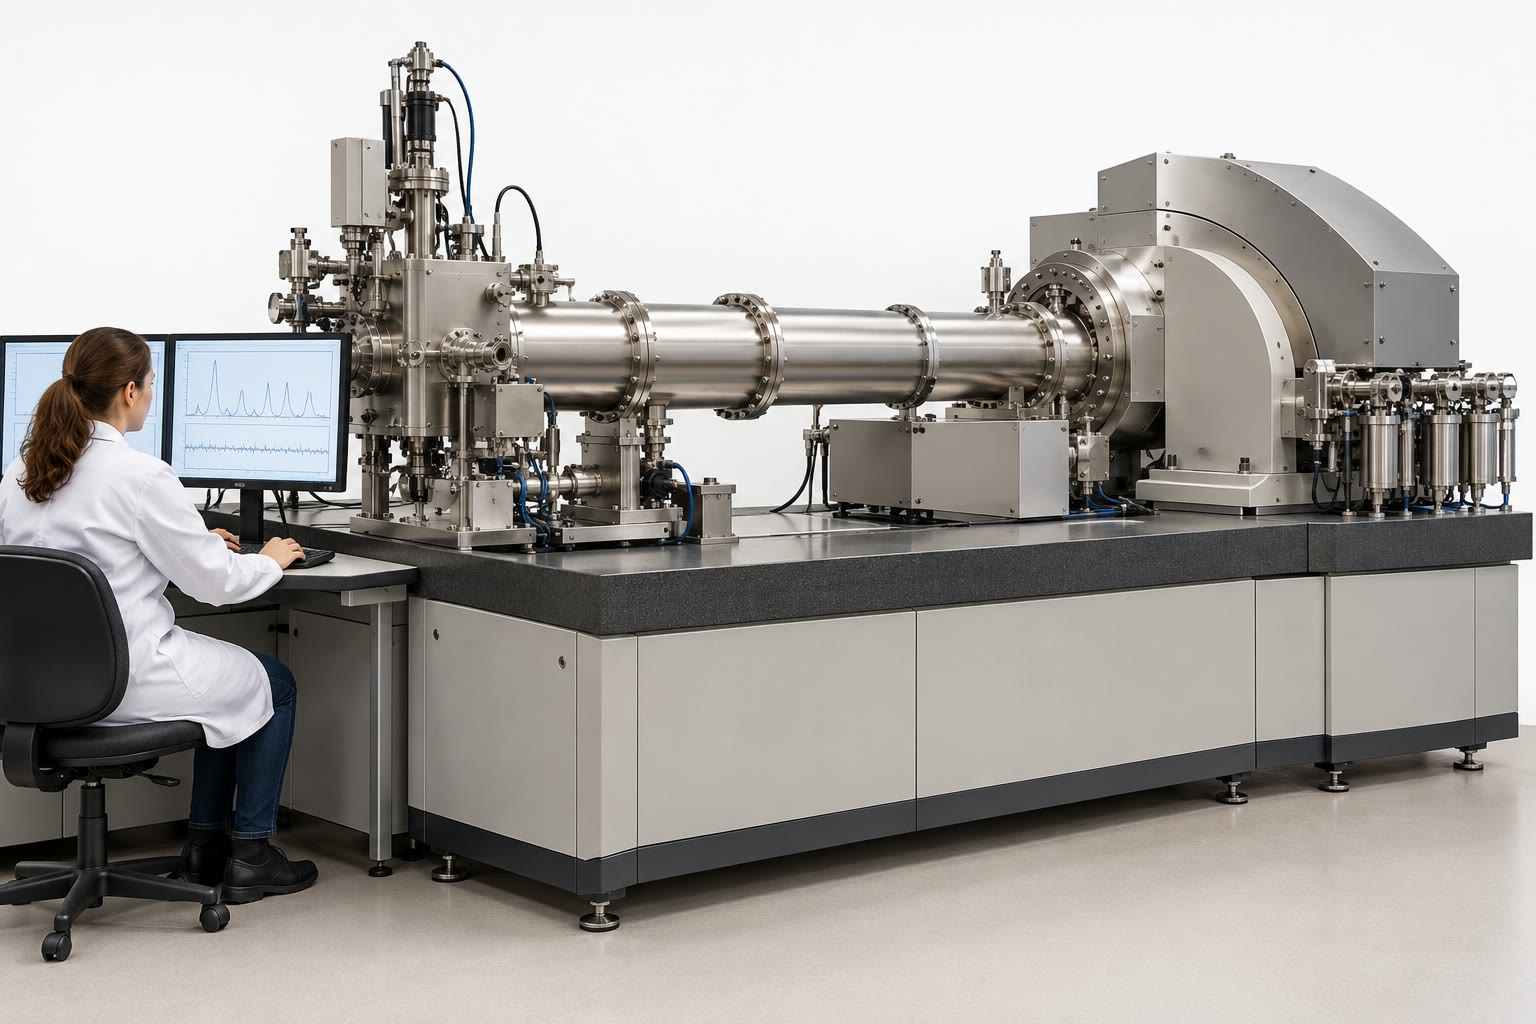
\includegraphics[width=\linewidth]{images/book4/ai/b2-isotope-lab.jpg}
\par\smallskip{\scriptsize مطياف كتلة متعدد المجمّعات في مختبر
للنظائر (رسم توضيحي مولَّد بالذكاء الاصطناعي).}
\end{minipage}
\end{inthelab}
% ledger: white:chur

\section{التمارين}

\begin{exercise}[$\star$]\label{exo:b2:isotope-geochemistry:1}
لبازلت من تريستان دا كونا $^{143}\mathrm{Nd}/^{144}\mathrm{Nd} = 0.51249$
ولآخر من مانغايا 0.51285. احسب $\varepsilon_{\mathrm{Nd}}$ لكل منهما ولبازلت MORB
المتوسط (0.513074). أيّ المصادر كانت لها نسبة Sm/Nd أعلى من الكوندريتات؟
\end{exercise}

\begin{exercise}[$\star$]\label{exo:b2:isotope-geochemistry:2}
النسبة $^{18}\mathrm{O}/^{16}\mathrm{O}$ هي \num{2.0052e-3} في \omterm{def:b2:isotope-geochemistry:standards}{VSMOW}
و\num{2.0672e-3} في \omterm{def:b2:isotope-geochemistry:standards}{VPDB}. ما قيمة $\delta^{18}\mathrm{O}$ للمعيار \omterm{def:b2:isotope-geochemistry:standards}{VPDB} على مقياس
\omterm{def:b2:isotope-geochemistry:standards}{VSMOW}؟ لكالسيت $\delta^{18}\mathrm{O} = -2.0$ بالجزء في الألف (\omterm{def:b2:isotope-geochemistry:standards}{VPDB})؛ احسب نسبته
وقيمة $\delta^{18}\mathrm{O}$ له على مقياس \omterm{def:b2:isotope-geochemistry:standards}{VSMOW}.
\end{exercise}

\begin{exercise}[$\star$]\label{exo:b2:isotope-geochemistry:3}
احسب $^{143}\mathrm{Nd}/^{144}\mathrm{Nd}$ للخزّان CHUR قبل \qty{1.0}{Ga}
وقبل \qty{4.567}{Ga} ($\lambda_{147} = \qty{6.524e-12}{\per\year}$،
$^{147}\mathrm{Sm}/^{144}\mathrm{Nd} = 0.1966$، واليوم 0.512638).
\end{exercise}

\begin{exercise}[$\star$]\label{exo:b2:isotope-geochemistry:4}
لعيّنة ثلج من محطة جبلية $\delta^{18}\mathrm{O} = -18.0$ بالجزء في الألف.
ما قيمة $\delta\mathrm{D}$ التي يتنبّأ بها \omterm{prop:b2:isotope-geochemistry:mwl}{خط الماء الجوي}؟ ولماء بحيرة
$\delta^{18}\mathrm{O} = -4.0$ و$\delta\mathrm{D} = -42$ بالجزء في الألف: احسب فائض
الديوتيريوم فيه $d = \delta\mathrm{D} - 8\delta^{18}\mathrm{O}$، واذكر هل يقع فوق
الخط أم تحته.
\end{exercise}

\begin{exercise}[$\star\star$]\label{exo:b2:isotope-geochemistry:5}
احسب $Q$ في قضية النموّ الخطي. لغرانيت Sm \qty{6.0}{ppm}
وNd \qty{30}{ppm} (CI: 0.145 و\qty{0.457}{ppm}). احسب
$f_{\mathrm{Sm/Nd}}$ له، وتغيّر $\varepsilon_{\mathrm{Nd}}$ فيه على مدى
\qty{500}{Myr}.
\end{exercise}

\begin{exercise}[$\star\star$]\label{exo:b2:isotope-geochemistry:6}
انفصلت قشرة قبل \qty{2.7}{Ga} عن وشاح له
$\varepsilon_{\mathrm{Nd}} = +3.5$، مع $f_{\mathrm{Sm/Nd}} = -0.45$. قدّر
$\varepsilon_{\mathrm{Nd}}$ لها اليوم بقضية النموّ الخطي. يعطي الحساب
الدقيق $-27.3$؛ فبكم يختلف التقريب، ولماذا هو
أعلى أو أدنى مما ينبغي؟
\end{exercise}

\begin{exercise}[$\star\star$]\label{exo:b2:isotope-geochemistry:7}
تتمثّل صهارة بازلتية (Sr \qty{130}{ppm}، $^{87}\mathrm{Sr}/^{86}\mathrm{Sr} = 0.7030$)
غرانيتًا (Sr \qty{320}{ppm}، 0.7200). احسب
$^{87}\mathrm{Sr}/^{86}\mathrm{Sr}$ لمزائج فيها 5 و10 و20 في المئة من الغرانيت.
بيّن أن $^{87}\mathrm{Sr}/^{86}\mathrm{Sr}$ خط مستقيم بدلالة $1/\mathrm{Sr}$
وأعطِ ميله ومقطعه.
\end{exercise}

\begin{exercise}[$\star\star$]\label{exo:b2:isotope-geochemistry:8}
مع معاملي التجزّؤ بين السائل والبخار 1.0098 (للنظير $^{18}$O) و1.084 (للديوتيريوم D) عند
\qty{20}{\degreeCelsius}، احسب $\delta^{18}\mathrm{O}$ و$\delta\mathrm{D}$ لبخار
متوازن مع ماء المحيط (0، 0)، وميل
$\delta\mathrm{D}/\delta^{18}\mathrm{O}$ للخط من الماء إلى البخار. وأعد الحساب
عند \qty{0}{\degreeCelsius} (1.0117 و1.111). وقارن \omterm{prop:b2:isotope-geochemistry:mwl}{بخط الماء الجوي}.
\end{exercise}

\begin{exercise}[$\star\star$]\label{exo:b2:isotope-geochemistry:9}
تمثّل القشرة القارية 0.51 في المئة من كتلة الأرض السيليكاتية وتحوي،
في المتوسط، \qty{27}{ppm} من Nd مقابل \qty{1.25}{ppm} للأرض السيليكاتية. خذ
$\varepsilon_{\mathrm{Nd}}$ للقشرة $-15$ وللأرض السيليكاتية 0. ما
حصّة القشرة من النيوديميوم؟ ولو كان بقية الوشاح متجانسًا،
فكم تكون $\varepsilon_{\mathrm{Nd}}$ له؟ وما حصّة النيوديميوم التي يجب أن يحويها
خزّان مستنزَف عند $+8.5$ إذا كان باقي الوشاح كوندريتيًا؟
\end{exercise}

\begin{exercise}[$\star\star\star$]\label{exo:b2:isotope-geochemistry:10}
بيّن أن الحدود المهملة في قضية النموّ الخطي حجمها النسبي
نحو $\lambda t/2$. فكم يبلغ ذلك على مدى عمر الأرض، وكم
يسبّب من خطأ في $\varepsilon_{\mathrm{Nd}}$ من أجل $f = -0.45$ على مدى
\qty{2.7}{Ga}؟
\end{exercise}

\begin{exercise}[$\star\star\star$]\label{exo:b2:isotope-geochemistry:11}
لمكوّنين نسبتا Sr/Nd تبلغان 13.3 (للمكوّن A) و5.0 (للمكوّن B). مستعينًا ببرهان
\omterm{prop:b2:isotope-geochemistry:mixing}{قطع المزج الزائد}، أوجد الحصّة $s'$ من السترونشيوم الآتية من A في مزيج يقدّم فيه A
حصّة $s = 0.5$ من النيوديميوم. ولأيّ قيمة للحصّة $s$ تختلف
الحصّتان أكثر ما يمكن؟
\end{exercise}

\begin{exercise}[$\star\star\star$]\label{exo:b2:isotope-geochemistry:12}
يعطي نموذج صناديق من 2.3 إلى 2.6 ضعف الحجم الحالي للقشرة القارية،
\qty{7.2e9}{km^3}، وُلّدت منذ تكوّن الأرض قبل \qty{4.5}{Ga}، ومن 1.3 إلى 1.6
ضعفه هُدم. احسب متوسطي معدلي التوليد والهدم بوحدة
\unit{km^3} في السنة. وقارنهما بالمعدلين الحاليين عند مناطق الاندساس،
\qty{2.7}{km^3} في السنة تُضاف و\qty{3.2}{km^3} في السنة تُزال.
\end{exercise}

\section{مسألة: ثلاث جزر، ثلاثة أوشحة}

\begin{problem}[{مسألة نهاية الأسبوع --- وضع حمم ثلاث جزر على
مصفوفة الوشاح، وفصل مزيج عن مكوّن ثالث، وتأريخ
الرسوب المعاد تدويره}]
\label{pb:b2:isotope-geochemistry:1}
تنبثق من ثلاث جزر بركانية في محيط متخيَّل، كورا وفيل وآشا، بازلتات
لها النسب النظائرية الواردة أدناه. ويمثّل جيوكيميائي مصادرها بمكوّنين:
وشاح مستنزَف مثل مصدر MORB (Sr \qty{10}{ppm}، Nd
\qty{0.75}{ppm}، $^{87}\mathrm{Sr}/^{86}\mathrm{Sr} = 0.70282$،
$^{143}\mathrm{Nd}/^{144}\mathrm{Nd} = 0.51307$) ورسوب قديم أعاده
الاندساس إلى الوشاح (Sr \qty{200}{ppm}، Nd \qty{40}{ppm}، $0.72000$، $0.51141$؛
$^{147}\mathrm{Sm}/^{144}\mathrm{Nd} = 0.110$، $^{87}\mathrm{Rb}/^{86}\mathrm{Sr} = 0.50$).
كورا: $0.70410$، $0.51278$؛ فيل: $0.70618$، $0.51242$؛ آشا: $0.70290$، $0.51288$
($^{87}\mathrm{Sr}/^{86}\mathrm{Sr}$، $^{143}\mathrm{Nd}/^{144}\mathrm{Nd}$). الخزّان CHUR اليوم:
$^{143}\mathrm{Nd}/^{144}\mathrm{Nd} = 0.512638$، $^{147}\mathrm{Sm}/^{144}\mathrm{Nd} =
0.1966$؛ $\lambda_{147} = \qty{6.524e-12}{\per\year}$، $\lambda_{87} =
\qty{1.3972e-11}{\per\year}$.

\medskip\noindent\textbf{الجزء الأول --- وضع الجزر.}
\begin{enumerate}
\item احسب $\varepsilon_{\mathrm{Nd}}$ للمكوّنين.
\item احسب $\varepsilon_{\mathrm{Nd}}$ للجزر الثلاث.
\item ضع التراكيب الخمسة على مخطّط نسبة Sr و$\varepsilon_{\mathrm{Nd}}$. أيّ
الجزر تقع في الجانب المُثرى من CHUR؟
\item لآشا تقريبًا نسبة السترونشيوم التي للوشاح المستنزَف لكن قيمة
$\varepsilon_{\mathrm{Nd}}$ أدنى بكثير. أين تقع بالنسبة إلى مصفوفة الوشاح، وأيّ
مجموعة جزر في الفصل تشبه؟
\item لماذا يمكن اعتبار النسب النظائرية للحمم نسبَ مصادرها،
مع أن نسب Sm/Nd وRb/Sr في الحمم تختلف كثيرًا عنها في مصادرها؟
\item حمم من كورا لها $^{147}\mathrm{Sm}/^{144}\mathrm{Nd} = 0.12$ وعمرها \qty{1}{Myr}.
فبكم ازدادت نسبة $^{143}\mathrm{Nd}/^{144}\mathrm{Nd}$ فيها منذ الانبثاق، بوحدات
إبسيلون؟ وهل لذلك أهمية؟
\end{enumerate}

\noindent\textbf{الجزء الثاني --- مزج المكوّنين.}
\begin{enumerate}[resume]
\item اكتب تركيز Nd ونسبة $^{143}\mathrm{Nd}/^{144}\mathrm{Nd}$ لمزيج
فيه كسر كتلي $f$ من الرسوب.
\item احسب $\varepsilon_{\mathrm{Nd}}$ لمزائج فيها $f = 0.5$ و1 و2 و5 في
المئة.
\item احسب $^{87}\mathrm{Sr}/^{86}\mathrm{Sr}$ للمزائج نفسها.
\item بيّن أن $^{87}\mathrm{Sr}/^{86}\mathrm{Sr}$ للمزائج خط مستقيم
بدلالة $1/\mathrm{Sr}$، وأعطِ ميله.
\item احسب $K = (\mathrm{Sr}/\mathrm{Nd})_{\text{الوشاح}}/(\mathrm{Sr}/\mathrm{Nd})_{\text{الرسوب}}$.
أيّ النسبتين، نسبة Sr أم نسبة Nd، تتحرّك نحو الرسوب أسرع كلما كبرت $f$؟
\item كم مرة يفوق الرسوب الوشاح في محتوى Nd، وفي محتوى Sr؟
فسّر بهذه الأرقام لماذا يزيح واحد في المئة من الرسوب
$\varepsilon_{\mathrm{Nd}}$ بنحو 11 وحدة.
\item ما حصّة نيوديميوم مزيج فيه $f = 1$ في المئة الآتية من
الرسوب؟
\end{enumerate}

\noindent\textbf{الجزء الثالث --- كم من الرسوب؟}
\begin{enumerate}[resume]
\item حلّ معادلة مزج Nd بالنسبة إلى $f$، إذا عُلمت النسبة $R$ للمزيج.
\item احسب $f$ لكورا من نيوديميومها.
\item احسب $f$ لكورا من سترونشيومها. هل يتّفق التقديران؟
\item احسب $f$ لفيل من نيوديميومها ومن سترونشيومها.
\item احسب $f$ لآشا من نيوديميومها، ونسبة السترونشيوم التي تتنبّأ بها
قيمة $f$ هذه. وقارن بالقيمة المقيسة: ماذا تستنتج عن مصدر
آشا؟
\item اقترح مكوّنًا ثالثًا لآشا، من الفصل، ونسب
الأم إلى الوليد التي لا بدّ أنها كانت له.
\end{enumerate}

\noindent\textbf{الجزء الرابع --- عمر الرسوب.}
\begin{enumerate}[resume]
\item اندسّ الرسوب قبل \qty{2.0}{Ga} وبقي مغلقًا منذ ذلك الحين.
احسب $^{143}\mathrm{Nd}/^{144}\mathrm{Nd}$ له، وللخزّان CHUR،
و$\varepsilon_{\mathrm{Nd}}$ له في ذلك الوقت.
\item أعد الحساب بقضية النموّ الخطي.
\item احسب $^{87}\mathrm{Sr}/^{86}\mathrm{Sr}$ للرسوب قبل \qty{2.0}{Ga}.
\item قبل \qty{2.0}{Ga} كانت لقشرة شكل $\varepsilon_{\mathrm{Nd}}$ قيمة
$\varepsilon_{\mathrm{Nd}} \approx -4.7$. هل تتّسق قيمة الرسوب عند الاندساس
مع نشأته بتعرية قشرة قارية فتيّة كهذه؟
\item اذكر الكسر الكتلي للرسوب المعاد تدويره في مصدر الجزيرة الأكثر
إثراءً، وهو الرقم الأساسي في هذه المسألة.
\end{enumerate}
\end{problem}
% ledger: white:chur, villa20:sm147, villa22:rb87, gale13:isotopes
